\begin{center}
  \textbf{Отчёт лабораторной работы №\envReportLabNumber}
\end{center}

\textbf{Тема}:
<<\envReportTitle>>

\begin{center}
  \textbf{Логическая модель}
\end{center}

Логическая модель изображена на рисунке~\ref{fig:logic_model}.

\begin{figure}[!h]
  \centering

  \includegraphics[width=21cm, angle=90]
  {../database/logic_model.pdf}

  \caption{Логическая модель}

  \label{fig:logic_model}
\end{figure}

\newpage

\begin{center}
  \textbf{Задание 1}
\end{center}

\textbf{Условие}:
Написать команду, которая вводит в таблицу SUBJECT строку для нового предмета обучения под названием “Алгебра”.
Читается этот предмет в четвертом семестре, отводится на него 72 часа,
ID этого предмета 201.

\begin{center}
  \textbf{Решение задания 1}
\end{center}

\lstinputlisting[language=sql, name={Данные заполненные не вводя ID}]
{../data/disciplines.sql}

\lstinputlisting[language=sql]{../sql/task1/1.sql}

\textbf{Результат}: вся выборка изображена на рисунке~\ref{fig:t1}.

\begin{figure}[!h]
  \centering

  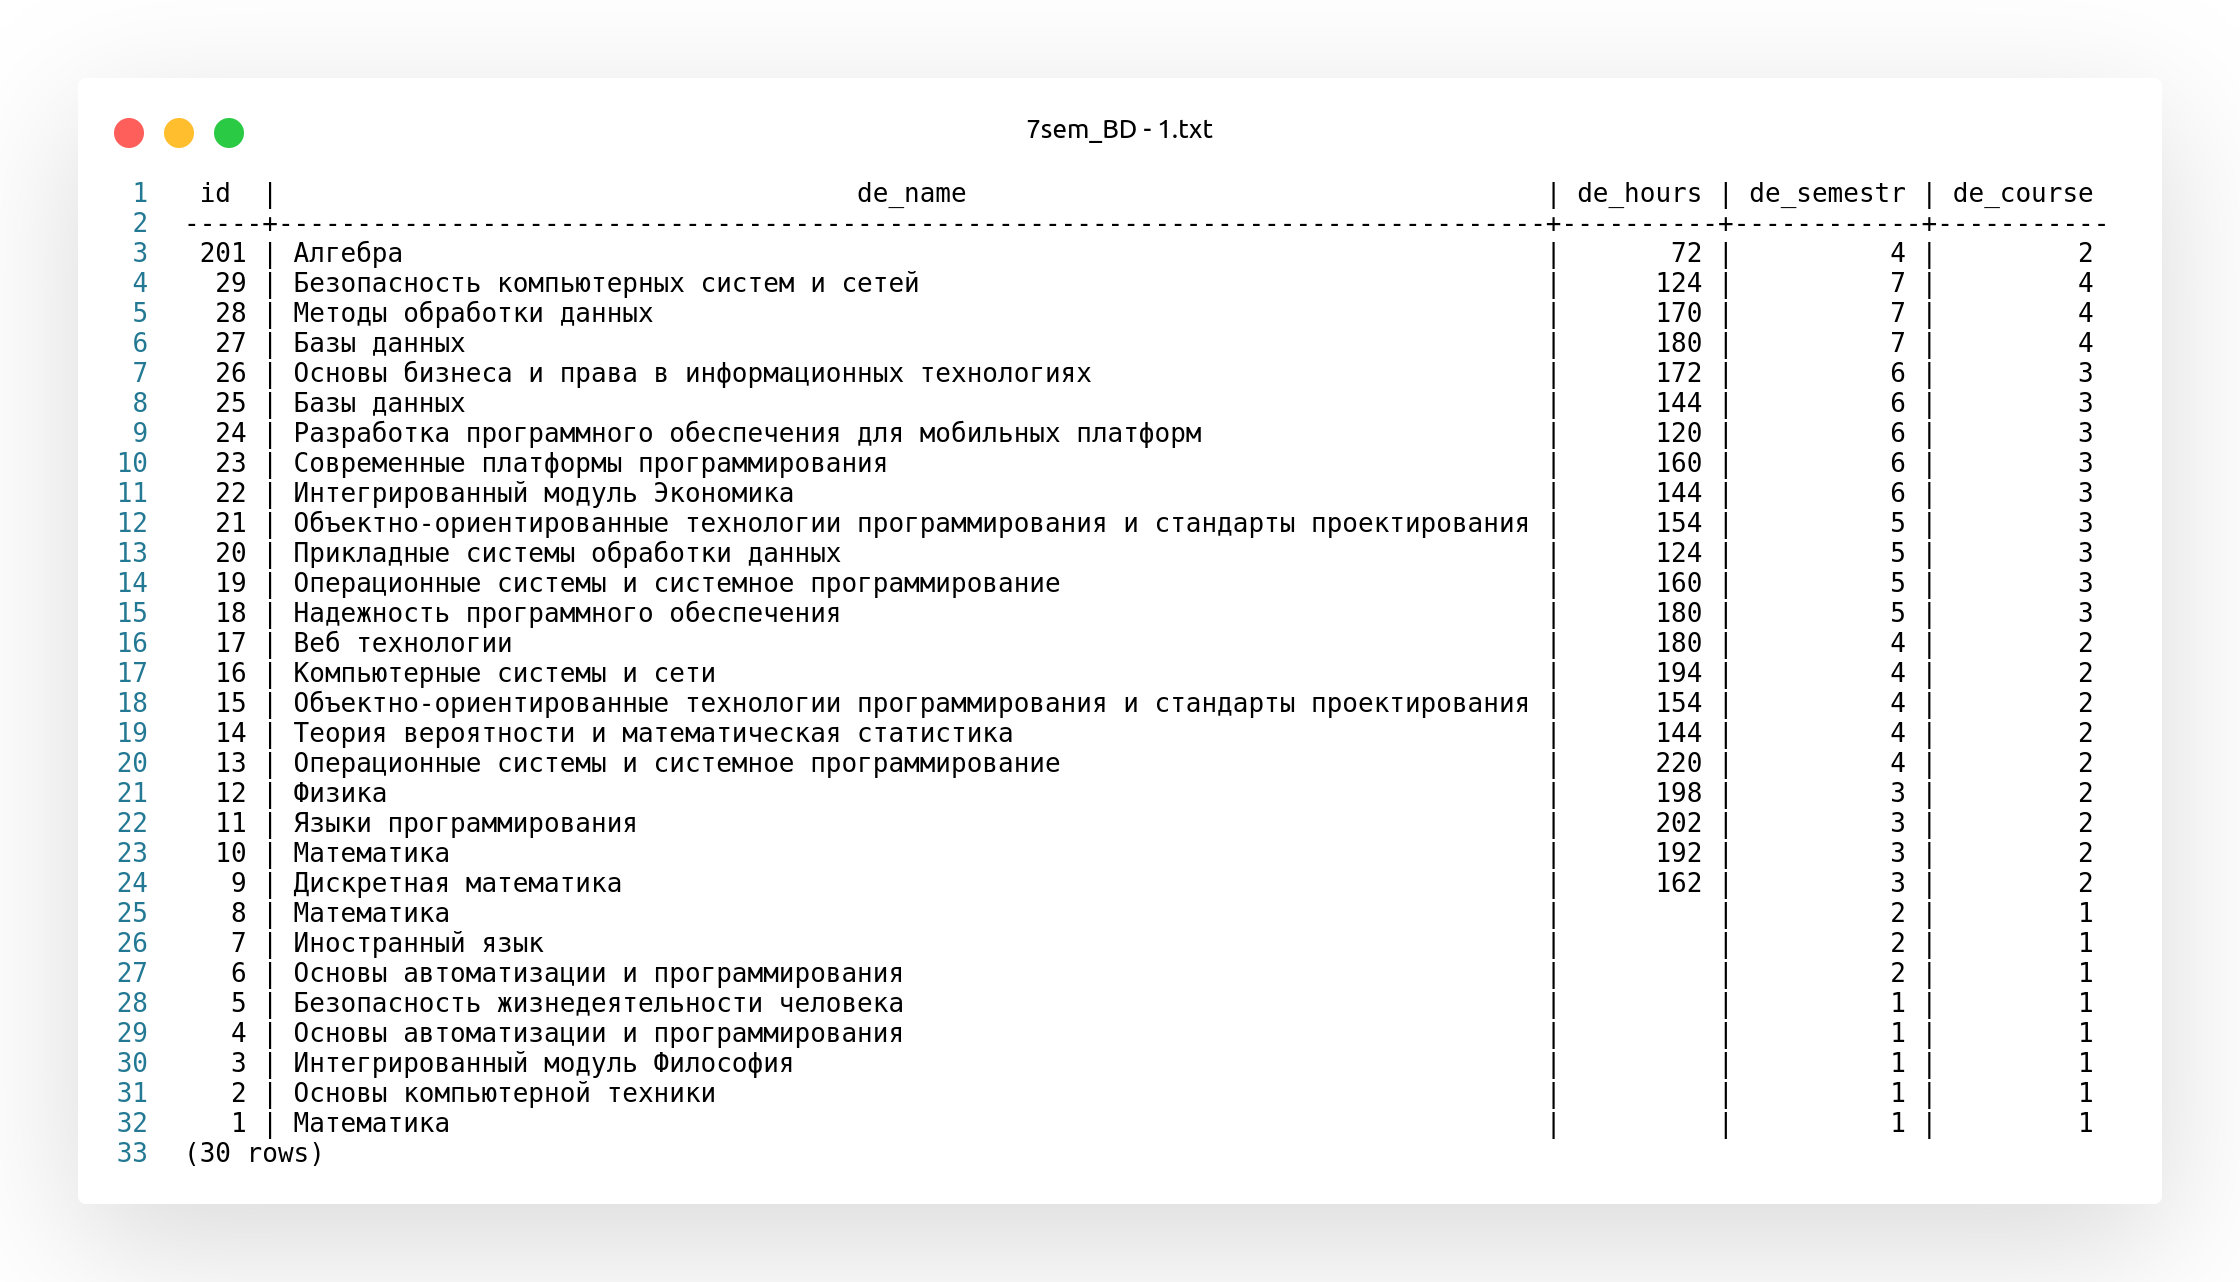
\includegraphics[width=18cm]
  {../sql/task1/1.png}

  \caption{Выборка из задания №1}

  \label{fig:t1}
\end{figure}

\newpage

\begin{center}
  \textbf{Задание 2}
\end{center}

\textbf{Условие}:
Напишите команду, которая увеличивает на 5\% значения всех рейтингов университетов,
в которых учатся более 1000 студентов.

\textbf{Результат}: вся выборка до UPDATE изображена на рисунке~\ref{fig:t2_1}
и вся выборка после UPDATE изображена на рисунке~\ref{fig:t2_2}.

\begin{figure}[!h]
  \centering

  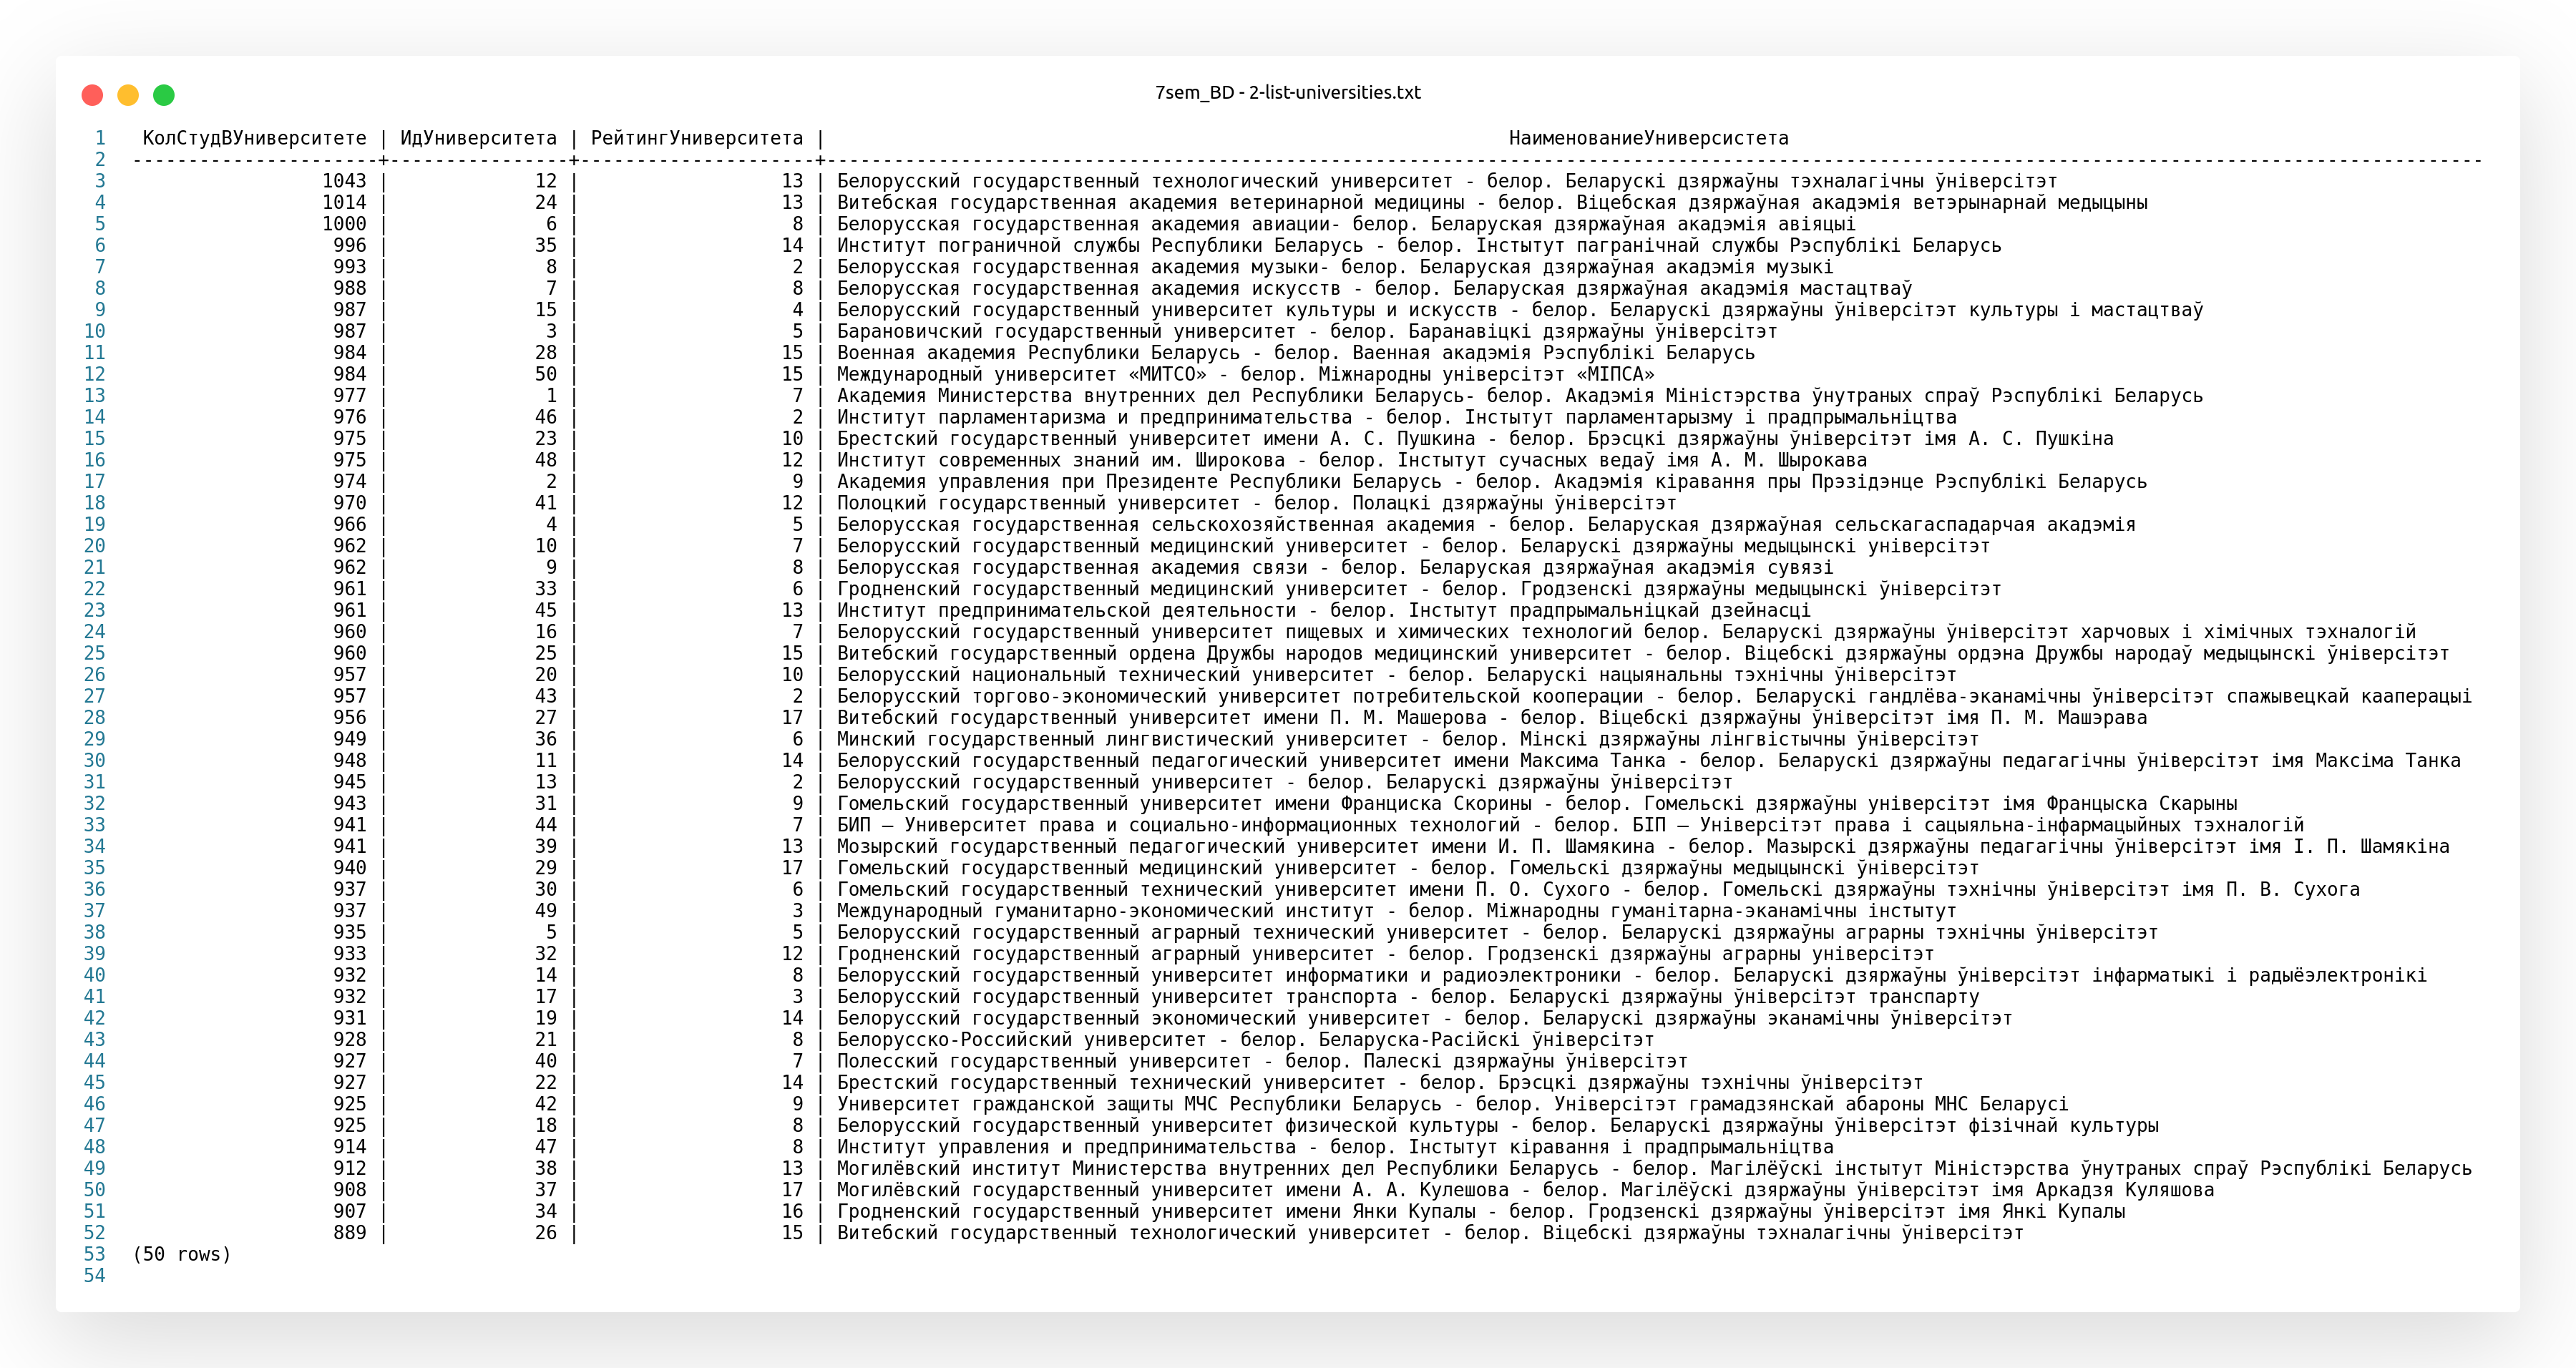
\includegraphics[width=18cm]
  {../sql/task2/2-list-universities__before.png}

  \caption{Выборка из задания №2 до UPDATE}

  \label{fig:t2_1}
\end{figure}

\lstinputlisting[language=sql]{../sql/task2/2.sql}

\begin{figure}[!h]
  \centering

  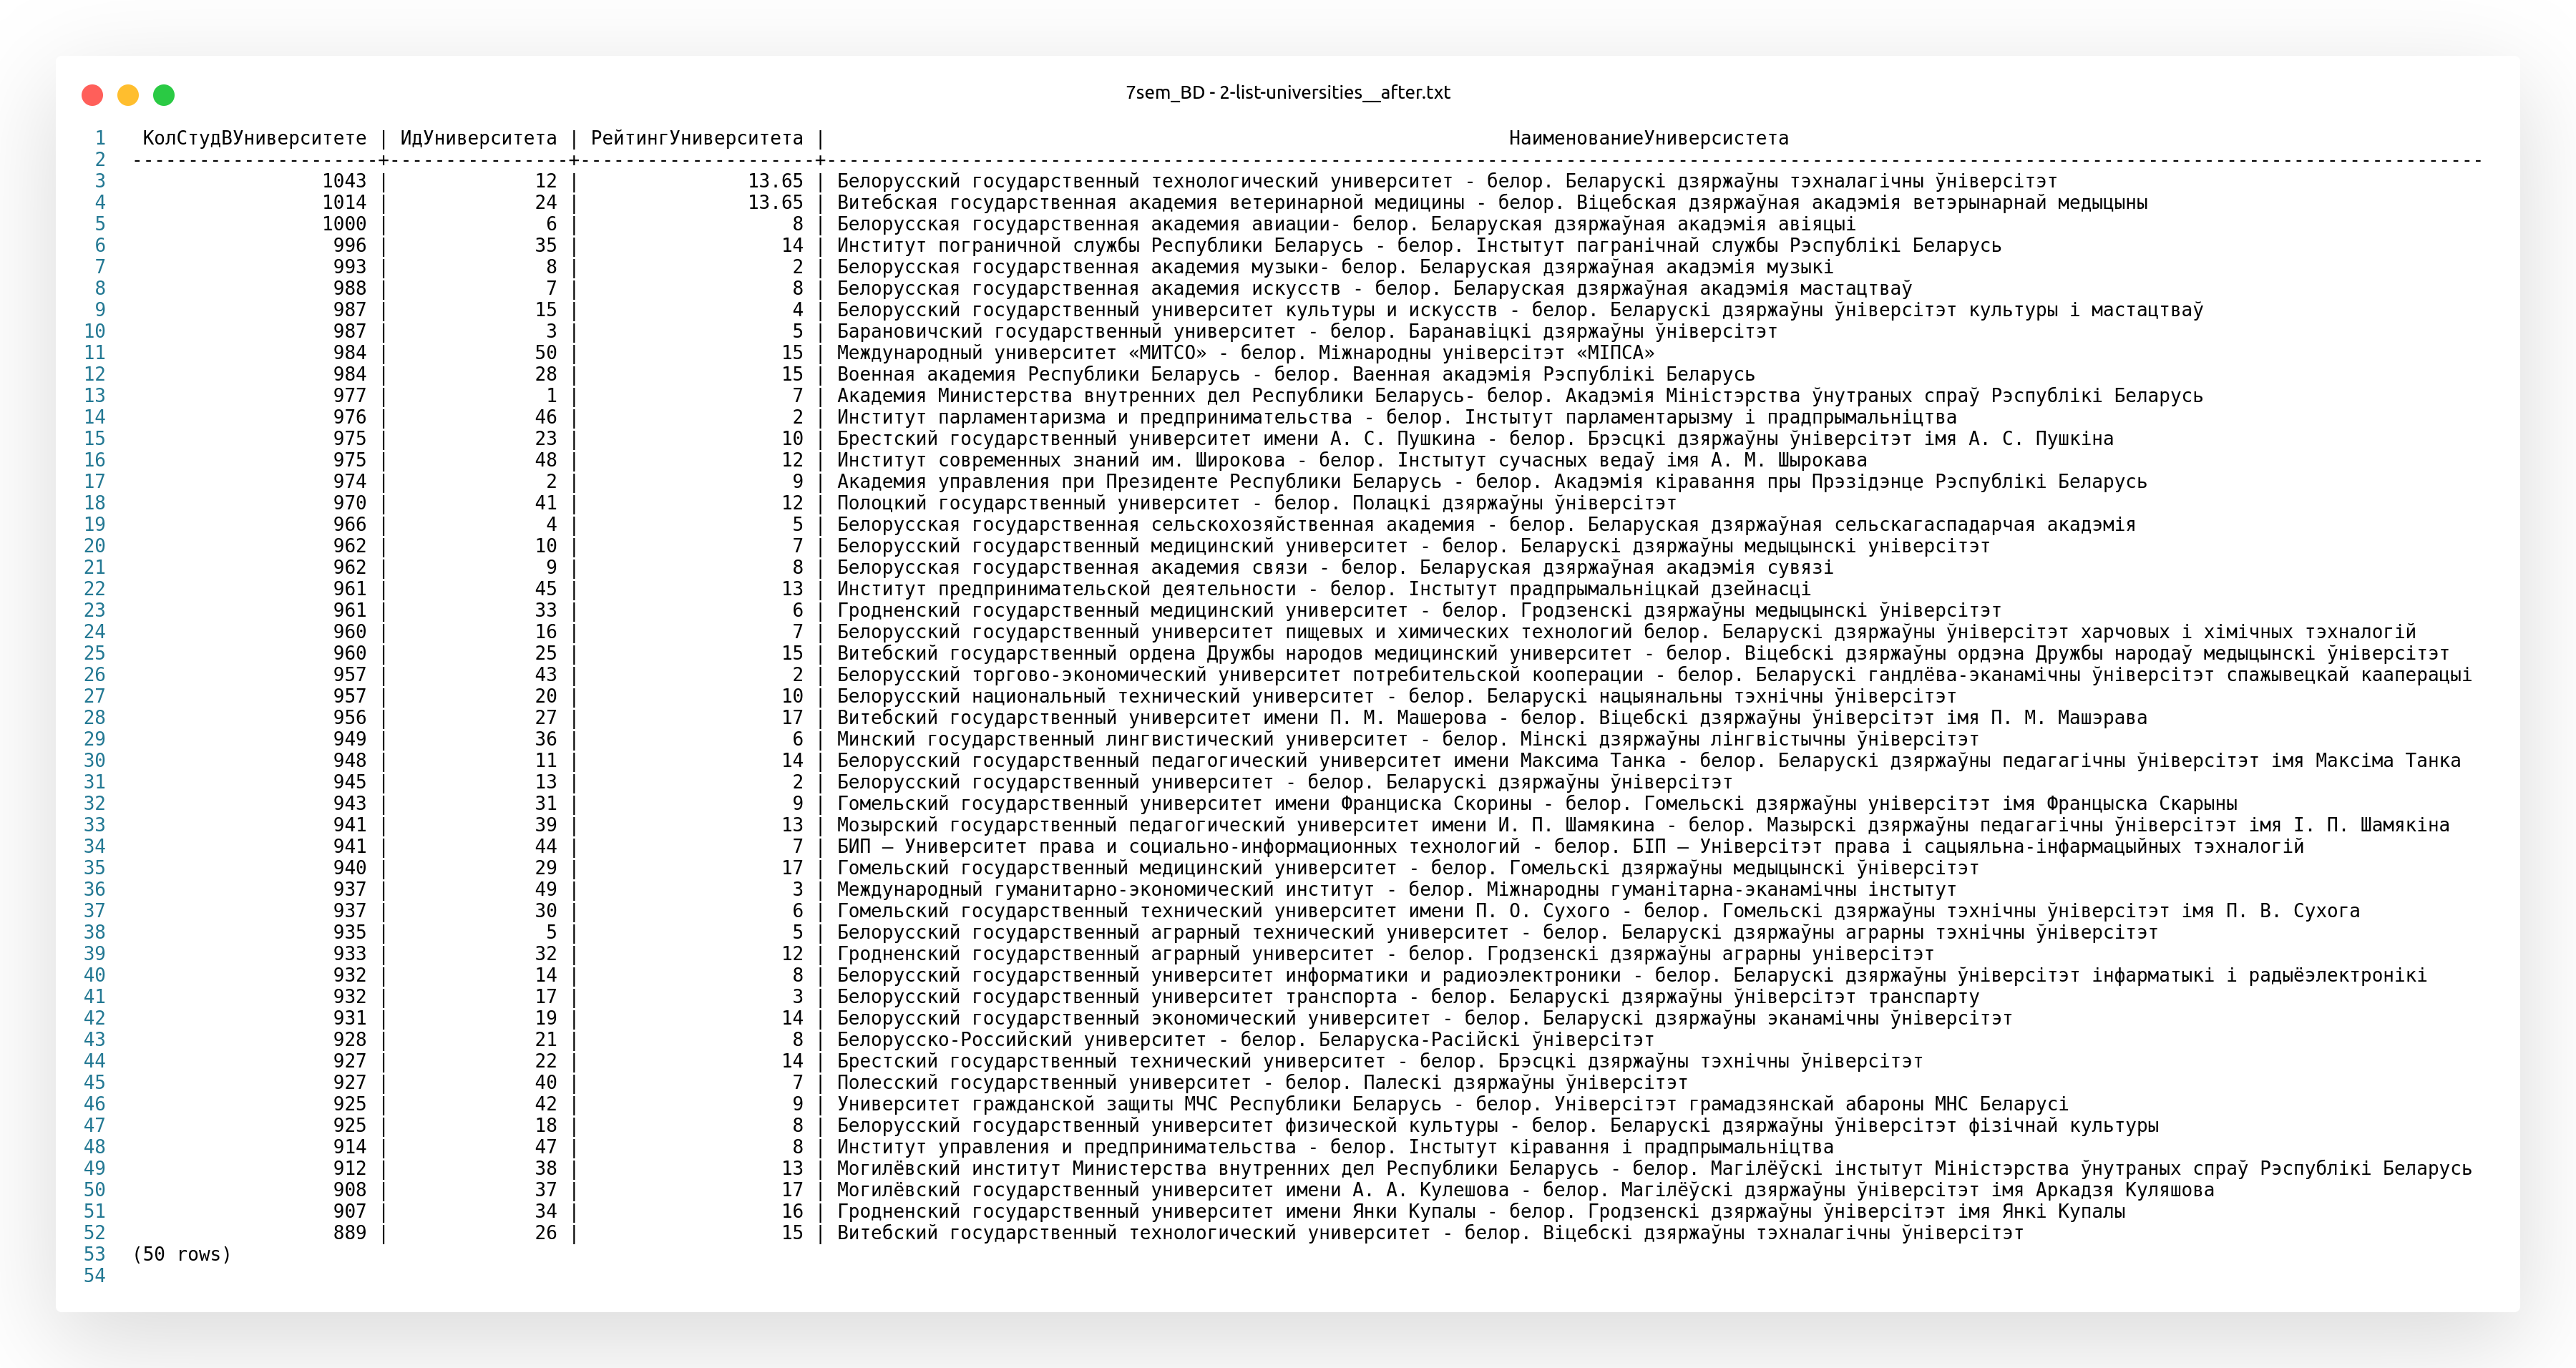
\includegraphics[width=18cm]
  {../sql/task2/2-list-universities__after.png}

  \caption{Выборка из задания №2 после UPDATE}

  \label{fig:t2_2}
\end{figure}

\lstinputlisting[language=sql, name={Скрипт, который выводил таблицу университетов ДО и ПОСЛЕ UPDATE}]
{../sql/task2/2-list-universities.sql}

\newpage

\begin{center}
  \textbf{Задание 3}
\end{center}

\textbf{Условие}:
Напишите команду, удаляющую записи обо всех оценках студентов,
среднее значение оценок которых ниже тройки.

\lstinputlisting[language=sql]{../sql/task3/3.sql}

\textbf{Результат}: вся выборка до DELETE изображена на рисунке~\ref{fig:t3_1}
и вся выборка после DELETE изображена на рисунке~\ref{fig:t3_2}.

\begin{figure}[!h]
  \centering

  \begin{minipage}{0.49\textwidth}
    \centering

    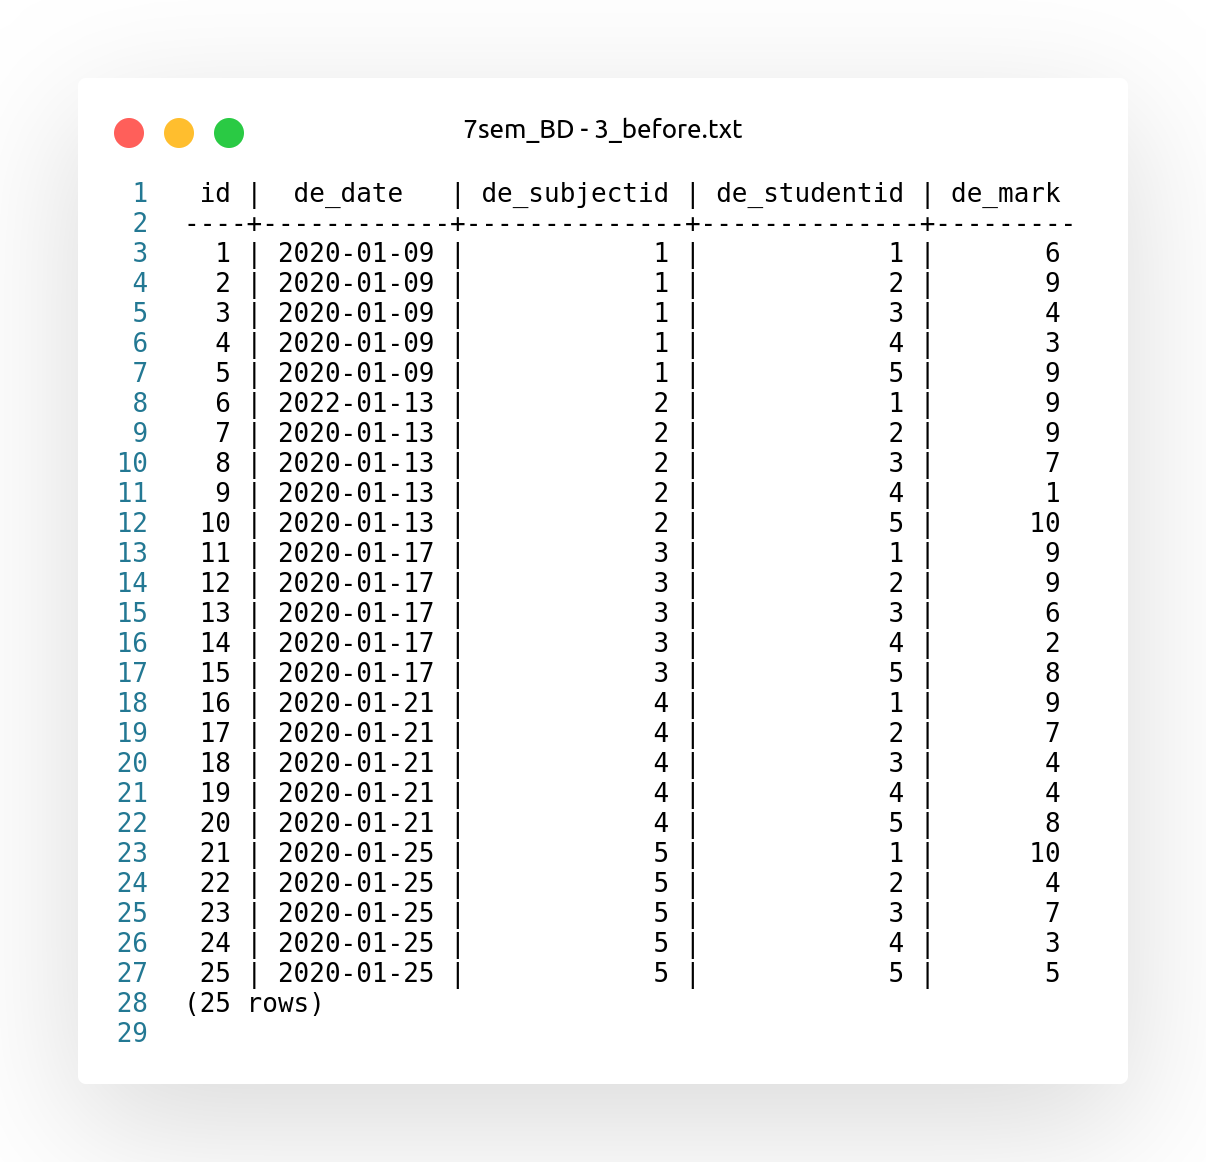
\includegraphics[width=7cm]
    {../sql/task3/3_before.png}

    \caption{До DELETE}
    \label{fig:t3_1}
  \end{minipage}
  \begin{minipage}{0.49\textwidth}
    \centering

    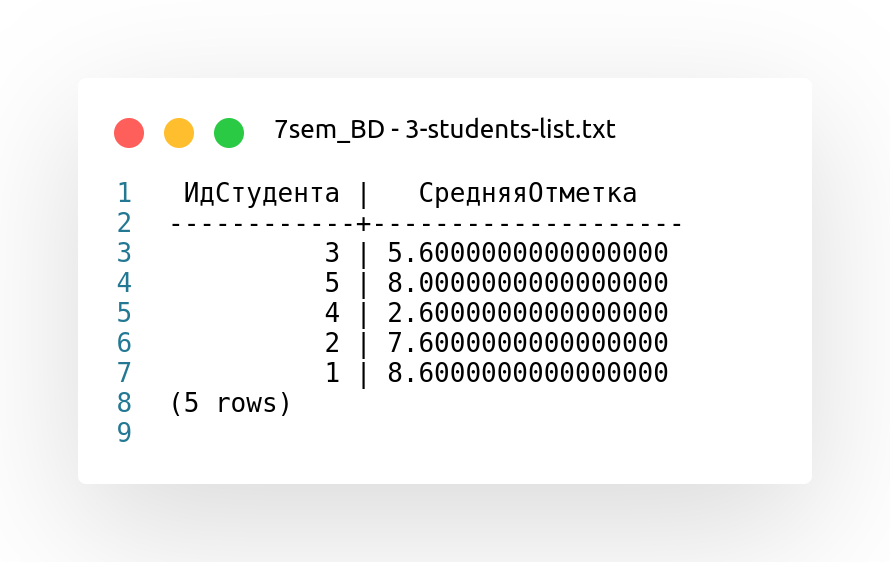
\includegraphics[width=8cm]
    {../sql/task3/3-students-list.png}

    \caption{Средняя отметка}
    \label{fig:t3_temp}
  \end{minipage}
  \begin{minipage}{0.49\textwidth}
    \centering

    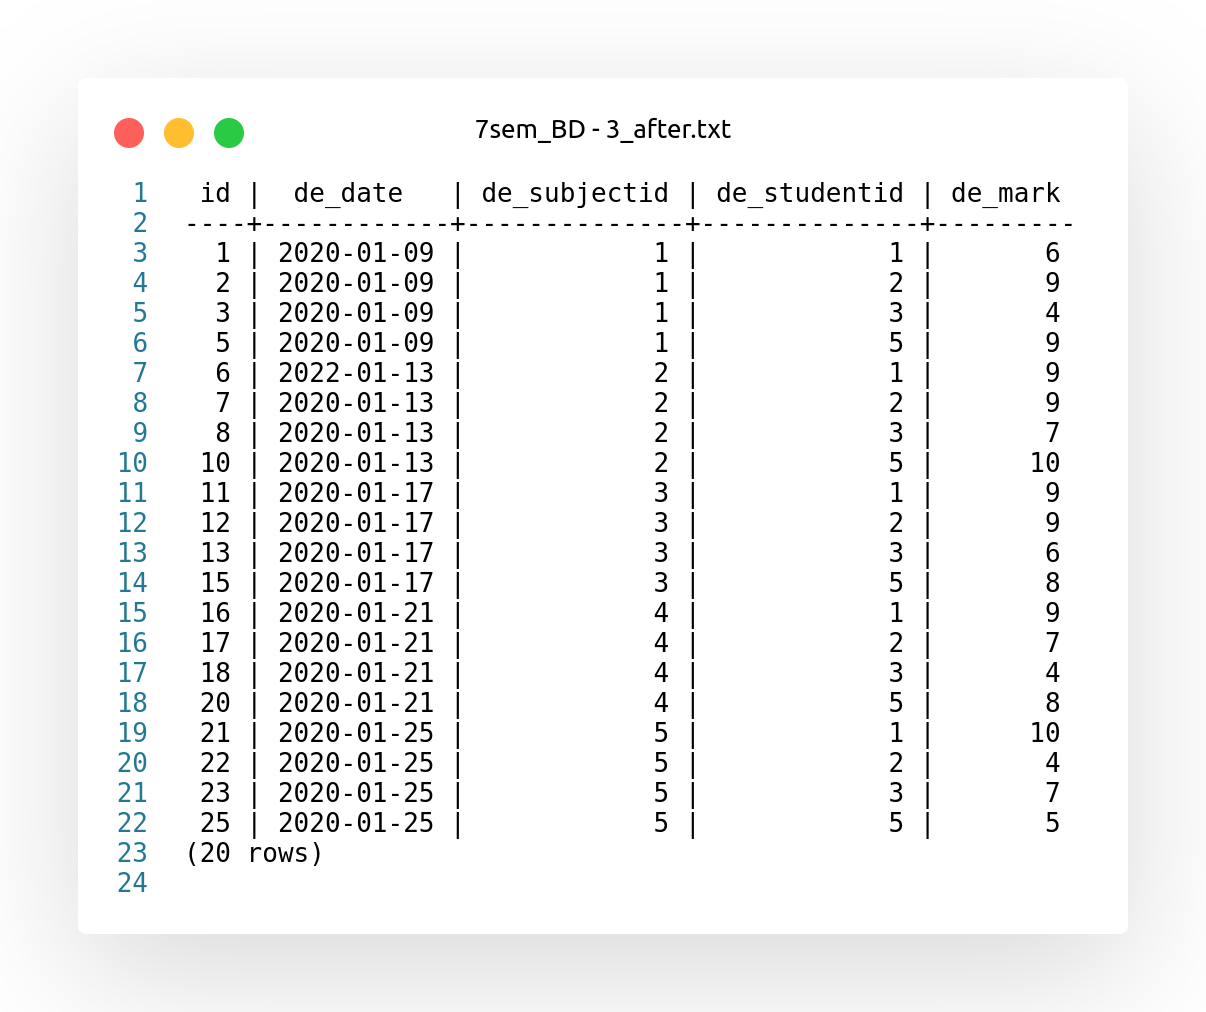
\includegraphics[width=7cm]
    {../sql/task3/3_after.png}

    \caption{После DELETE}
    \label{fig:t3_2}
  \end{minipage}
\end{figure}

\newpage

\begin{center}
  \textbf{Задание 4}
\end{center}

\textbf{Условие}:
Создать представление, позволяющее следить на каждый день сдачи экзаменов за количеством сданных экзаменов,
количеством студентов, сдавших эти экзамены и средним баллом.

\lstinputlisting[language=sql]{../sql/task4/4.sql}

\textbf{Результат}: вся выборка изображена на рисунке~\ref{fig:t4}.

\begin{figure}[!h]
  \centering

  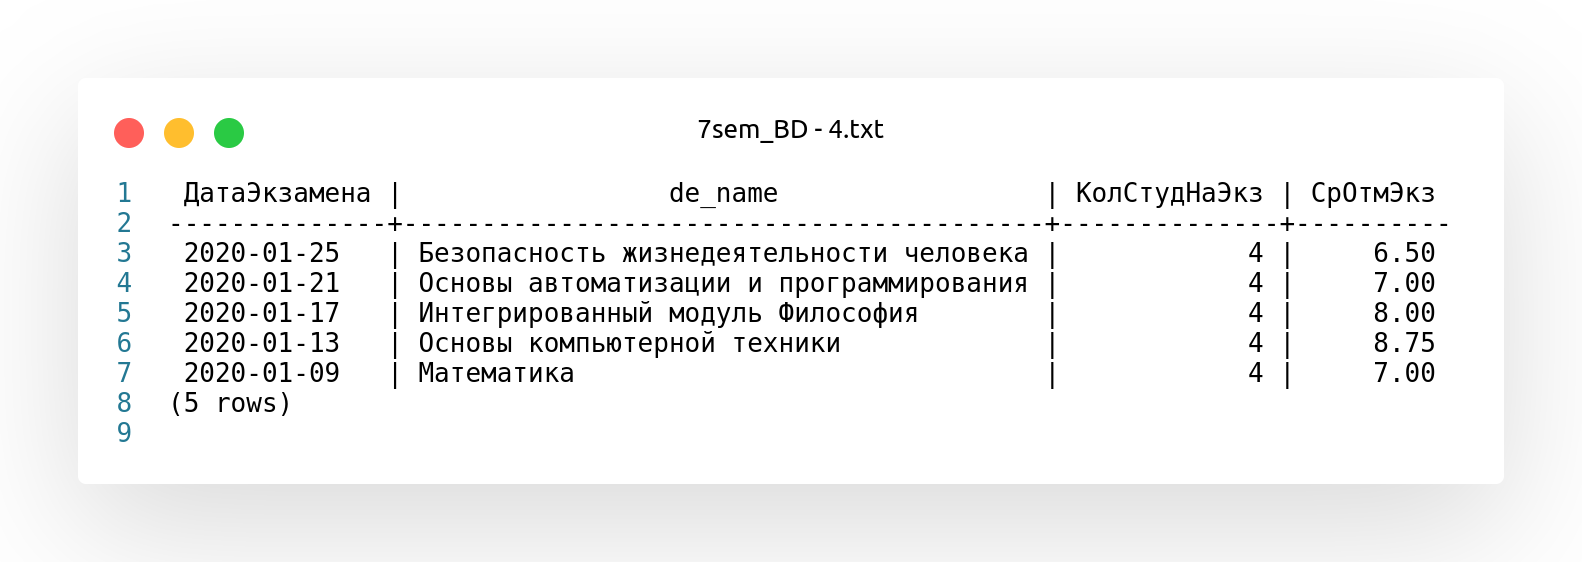
\includegraphics[width=18cm]
  {../sql/task4/4.png}

  \caption{Выборка из задания №4}

  \label{fig:t4}
\end{figure}

\newpage

\begin{center}
  \textbf{Задание 5}
\end{center}

\textbf{Условие}:
Создать представление, которое показывает имена
и названия сданных предметов для каждого студента

\lstinputlisting[language=sql]{../sql/task5/5.sql}

\textbf{Результат}: вся выборка изображена на рисунке~\ref{fig:t5}.

\begin{figure}[!h]
  \centering

  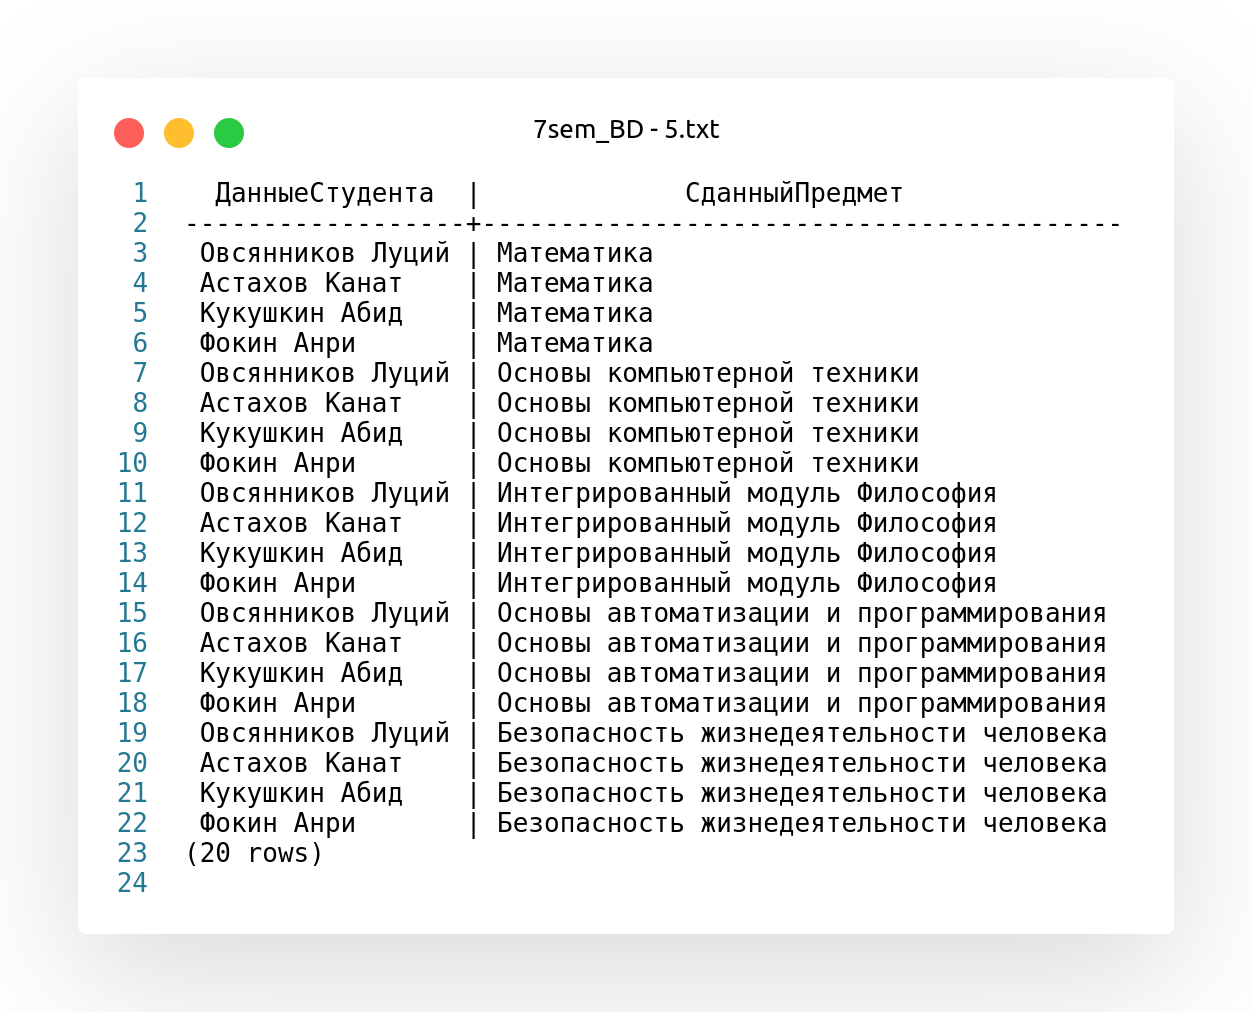
\includegraphics[height=13cm]
  {../sql/task5/5.png}

  \caption{Выборка из задания №5}

  \label{fig:t5}
\end{figure}

\newpage

\begin{center}
  \textbf{Задание 6}
\end{center}

\textbf{Условие}:
Создать представление, отображающее фамилию, имя, балл и дату получения оценки студентов,
имеющих самый высокий балл на каждую дату сдачи экзаменов.

\lstinputlisting[language=sql]{../sql/task6/6.sql}

\textbf{Результат}: вся выборка изображена на рисунке~\ref{fig:t6}.

\begin{figure}[!h]
  \centering

  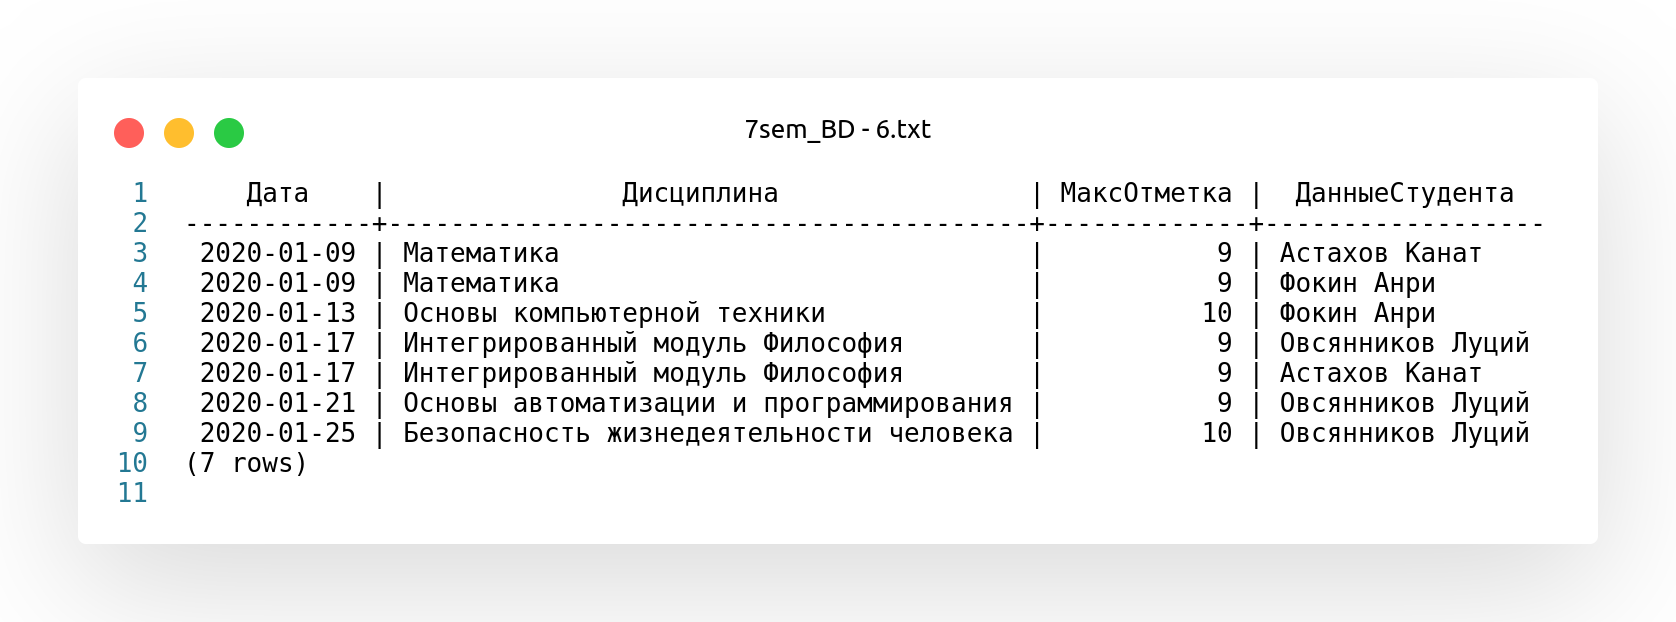
\includegraphics[width=18cm]
  {../sql/task6/6.png}

  \caption{Выборка из задания №6}

  \label{fig:t6}
\end{figure}

\newpage

\begin{center}
  \textbf{Задание 7}
\end{center}

\textbf{Условие}:
На основе предыдущего представления, создать новое представление, выводящее фамилии студентов,
имеющих самый высокий балл как минимум 3 раза.

\lstinputlisting[language=sql]{../sql/task7/7.sql}

\textbf{Результат}: вся выборка изображена на рисунке~\ref{fig:t7}.

\begin{figure}[!h]
  \centering

  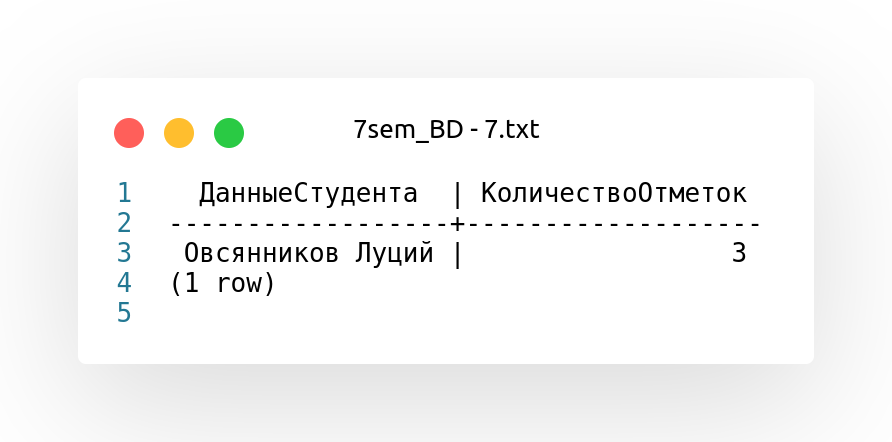
\includegraphics[width=12cm]
  {../sql/task7/7.png}

  \caption{Выборка из задания №7}

  \label{fig:t7}
\end{figure}

\newpage

\begin{center}
  \textbf{Задание 8}
\end{center}

\textbf{Условие}:
Создать представление, выводящее фамилии, имена и стипендии студентов,
имеющих величину стипендии в пределах от 100 до 600,
и позволяющее изменять и вводить значения стипендии только в этом интервале. 

\lstinputlisting[language=sql]{../sql/task8/8.sql}

\begin{figure}[!h]
  \centering

  \begin{minipage}{0.49\textwidth}
    \centering

    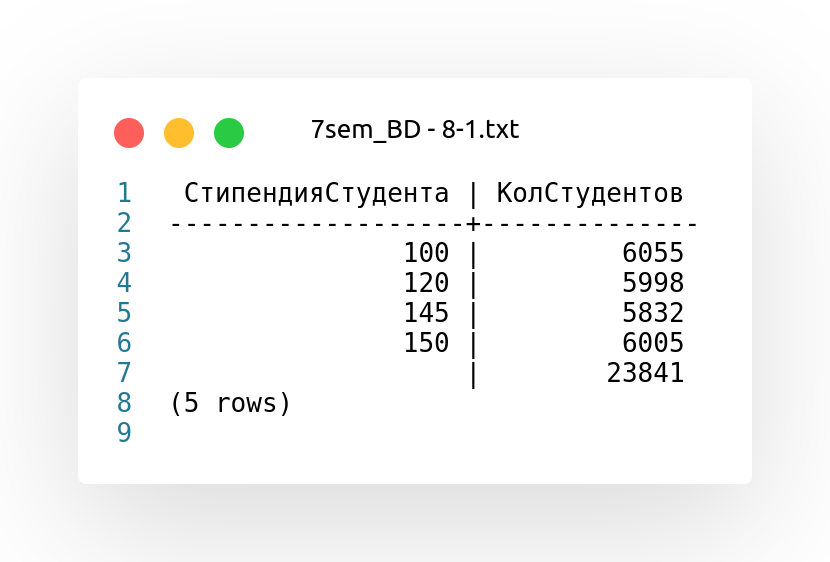
\includegraphics[width=8cm]
    {../sql/task8/8-1.png}

    \caption{Количество стипендий всей выборки}
    \label{fig:t8_1}
  \end{minipage}
  \begin{minipage}{0.49\textwidth}
    \centering

    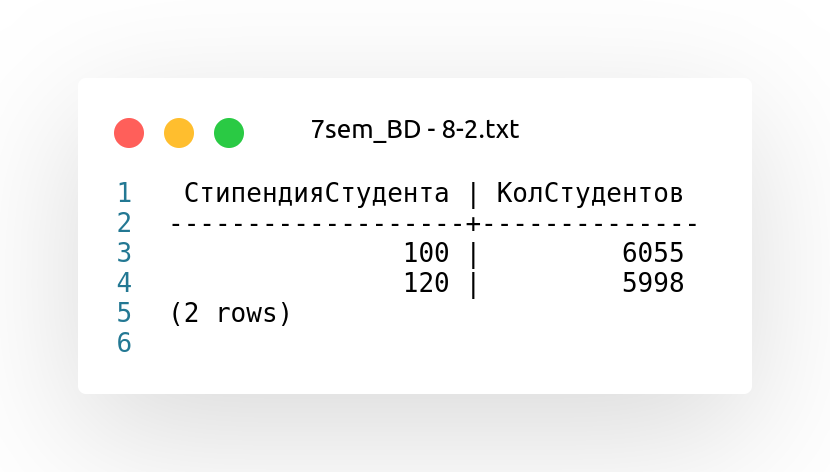
\includegraphics[width=8cm]
    {../sql/task8/8-2.png}

    \caption{Количество стипендий ограниченной выборки}
    \label{fig:t8_2}
  \end{minipage}
\end{figure}